\documentclass[useAMS, usenatbib]{mnras}
\pdfsuppresswarningpagegroup=1
%
\usepackage[spanish,es-minimal,english]{babel}
\usepackage[utf8]{inputenc}
\usepackage{graphicx}

\usepackage{xcolor}
\usepackage{hyperref}
\usepackage{siunitx}
\usepackage{newtxtext}
\usepackage[stix2,smallerops]{newtxmath}
\usepackage{booktabs}
\hypersetup{colorlinks=True, linkcolor=blue!50!black, citecolor=black,
  urlcolor=blue!50!black}
\usepackage{etoolbox}
\robustify\bfseries
\robustify\itshape

\usepackage[shortlabels]{enumitem}

\bibliographystyle{mnras}

\sisetup{
  % explicit "+" is useful for velocities
  retain-explicit-plus = true,
  % prefer 10^6 over 1 x 10^6
  retain-unity-mantissa = false,
  % Use x +/- e instead of x(e)  
  separate-uncertainty = true,
  % Make sure to pick up bold font when used in section heading for instance
  detect-weight = true,
}
\DeclareSIUnit\msun{\text{M\ensuremath{_\odot}}}
\DeclareSIUnit\lsun{\text{L\ensuremath{_\odot}}}

%%
%% Will macros
%%
% A better \ion command that works in more circumstances
\newcommand\ION[2]{#1\,\scalebox{0.9}[0.8]{\uppercase{#2}}}
\newcounter{ionstage}
\renewcommand{\ion}[2]{\setcounter{ionstage}{#2}% 
  \ensuremath{\mathrm{#1\,\scriptstyle\Roman{ionstage}}}}
\newcommand\hii{\ion{H}{2}}
\newcommand\nii{[\ion{N}{2}]}
\newcommand\oiii{[\ion{O}{3}]}
\newcommand\oii{[\ion{O}{2}]}
\newcommand\Wav[1]{\ensuremath{\lambda #1}}
% Chemical formulae
\newcommand*\chem[1]{\ensuremath{\mathrm{#1}}}

\newcommand\Fion{\ensuremath{F_{\text{ion}}}}
\newcommand\ionpar{\ensuremath{U_{\text{ion}}}}

\title[Permitted C II lines in the Orion Nebula]{
  \boldmath
  Carbon shines in starlight:
  Orion Nebula's inner rim\\
  revealed by \ion{C}{2} fluorescence
  % Shiny red carbon:
  % starlight fluorescence of \ion{C}{2}
  % reveals the inner rim of the Orion Nebula
}

\author[Henney et al.]{%
  William J. Henney,\(^1\)\thanks{
    w.henney@irya.unam.mx
  }
  % J. Garc{\'{\i}}a-Rojas,\(^{2,3}\)
  J. E. M\'endez-Delgado,\(^{2,3}\)
  % C. Esteban,\(^{2,3}\)
  % \newauthor 
  % A. Mesa-Delgado,\(^{4}\)
  % K. Z. Arellano-C\'ordova,\(^{2}\)
  % and 
  % M. Núñez-Díaz\(^{4}\)
  \\
  \(^1\)\foreignlanguage{spanish}{
    Instituto de Radioastronomía y
    Astrofísica, Universidad Nacional Autónoma de México, Apartado
    Postal 3-72, 58090 Morelia, Michaoacán, Mexico}
  \\
  \(^2\)\foreignlanguage{spanish}{
    Instituto de Astrof\'isica de Canarias (IAC), E-38205 La Laguna, Spain}
  \\
  \(^3\)\foreignlanguage{spanish}{
    Departamento de Astrof\'isica, Universidad de La Laguna, E-38206 La Laguna, Spain}
  % \\
  % \(^4\)\foreignlanguage{spanish}{
  %    Domicilio Particular, Tenerife, Spain}
}
% These dates will be filled out by the publisher
\date{Accepted XXX. Received YYY; in original form ZZZ}

% Enter the current year, for the copyright statements etc.
\pubyear{2020}

\begin{document} 
\label{firstpage}
\pagerange{\pageref{firstpage}--\pageref{lastpage}}
\maketitle

\begin{abstract}
  Lots of \ion{C}{2} lines. 
\end{abstract}


\begin{keywords}
  Atomic physics
  -- H II regions
  -- Radiative transfer
  -- techniques: imaging spectroscopy
\end{keywords}

\maketitle

\section{Introduction}
\label{sec:introduction}


% \begin{figure}
%   \centering
%   \includegraphics[width=\linewidth]{figs/oii-emissivity-vs-t}
%   \caption{Emissivities of different \chem{O^{++}} lines versus temperature.}
%   \label{fig:emissivities}
% \end{figure}

Calculations of recombination spectrum \citep{Pequignot:1991a, Davey:2000a}.
Calculation of fluorescent and recombination spectrum for a particular source (PN IC~418) by \citet{Escalante:2012a}.
Similar calculation for Orion Nebula, but for the \ion{N}{2} lines \citep{Escalante:2005a}. 

Rich spectrum of \ion{C}{2} observed in stellar wind of Wolf Rayet star in LMC \citep{Williams:2021s}. 

Rydberg Enhanced Recombination \citep{Nemer:2019a} may enhance the abundance of \chem{C^+} in the ionized interior of the nebula.  But note that we do not detect the signature 7115 line in Orion.

\begin{figure*}
  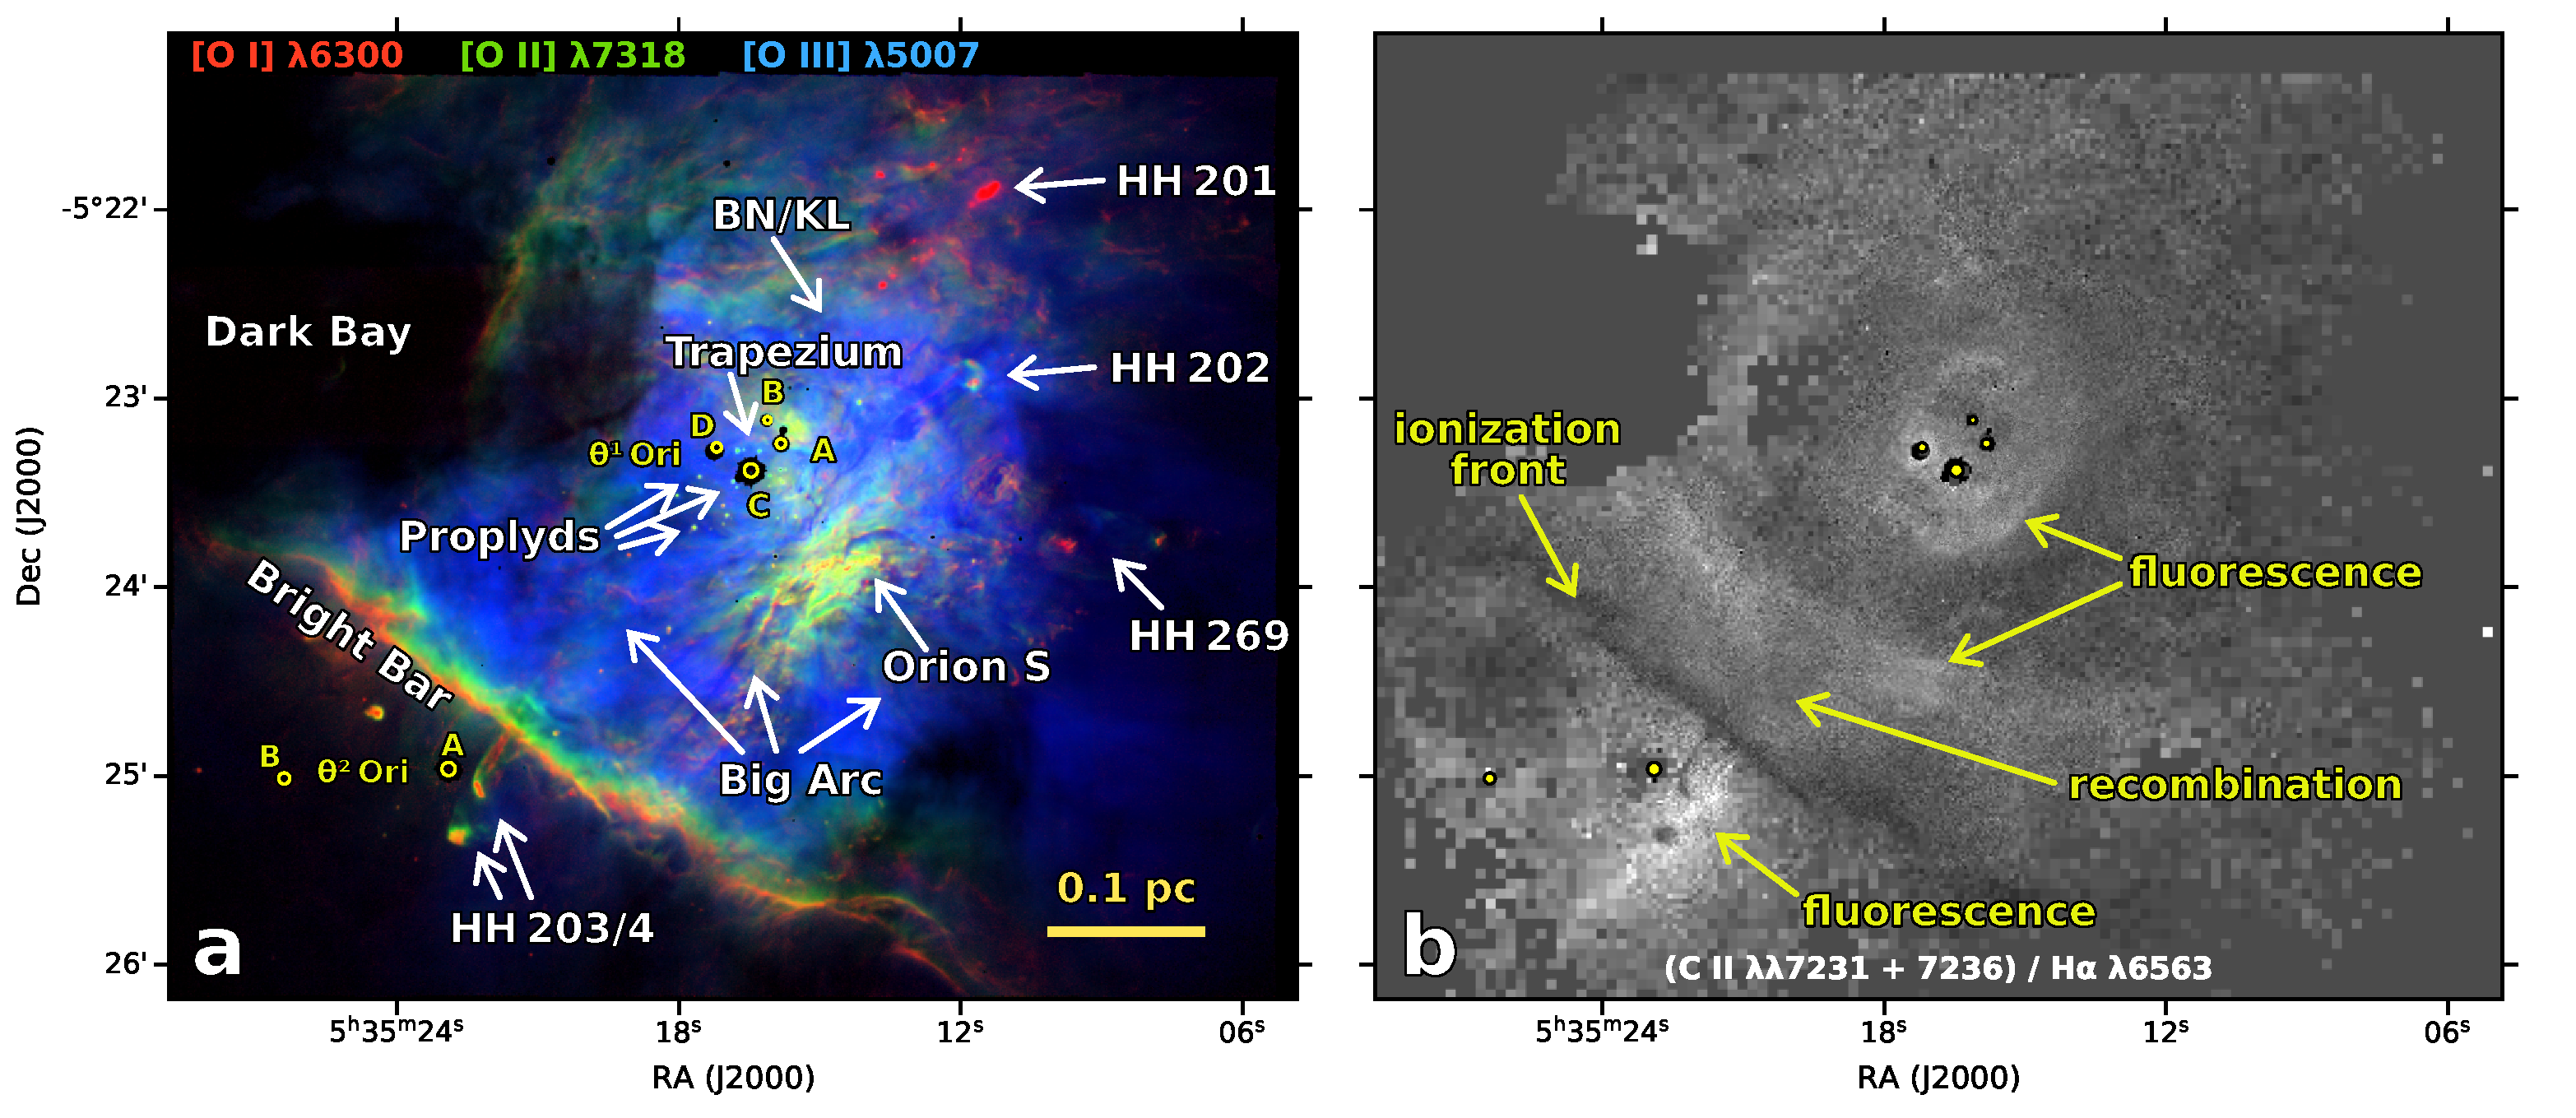
\includegraphics[width=\linewidth]{figs/rgb-plus-732x-ha-ratio-annotated}
  \caption{RGB image plus ratio image}
  \label{fig:rgb-plus-ratio}
\end{figure*}
\section{MUSE observations of Orion}
\label{sec:muse-observ-orion}

% \begin{figure}
%   \centering
%   \includegraphics[width=\linewidth]{figs/adal-slit6-oii-v1-annotated}
%   \caption{High-resolution ISIS-WHT spectra}
%   \label{fig:adal-pink-spectra}
% \end{figure}

% \begin{figure*}
%   \centering
%   \includegraphics[width=\linewidth]{figs/oii-v1-extraction-workflow}
%   \caption{Workflow for analyzing MUSE \ion{O}{2} spectral maps.  }
%   \label{fig:muse-workflow}
% \end{figure*}



\section{Discussion}
\label{sec:discussion}


\subsection{Nature of the Big Arc}
\label{sec:nature-big-arc}

\paragraph{Jet hypothesis}
That the Big Arc is the low-velocity sheath
that surrounds two separate wiggling stellar jets.

Other jet sources that show core-sheath structure.
HH~900 in Carina \citep{Reiter:2015a}
has a narrow jet in [\ion{Fe}{2}] and a broader, slower outflow in \ha{}.

Also molecular outflows are slower and less well collimated
than the jets, which are hypothesised to drive them. 

Two possibilities

\paragraph{Wind--bar interaction hypothesis}
That the Big Arc is a shell formed by the interaction between
the photoevaporation flow from the Orion Bar
and the Trapezium wind bubble.

Evidence in favor is the continuity in the PV diagrams between the high velocity and the lower-velocity bar emission.
And the fact that the lower-velocity component is only to the S of the Arc. 



% Other \ion{H}{2} regions.

% Planetary nebulae with moderate ADF.
% For instance the Ring Nebula \citep{Garnett:2001a} shows \ion{O}{2}~V1 peaking just inside [\ion{O}{3}],
% which is what one would expect from fluorescence. 


% Planetary nebulae with high ADF.
% I don't think there is any evidence for fluorescence being important in this case.
% \citet{Fang:2013a} have the lowest temperatures from \ion{O}{2} 3d--4f,
% which is consistent with cold clumps.

\section{Conclusions}
\label{sec:conclusions}


\bibliography{cii-orion-refs}


% Don't change these lines
\bsp	% typesetting comment
\label{lastpage}

\end{document}


%%% Local Variables:
%%% mode: latex
%%% TeX-master: t
%%% End:
